\documentclass{report}

\documentclass[12pt]{article}
\usepackage{array}
\usepackage{color}
\usepackage{amsthm}
\usepackage{eufrak}
\usepackage{lipsum}
\usepackage{pifont}
\usepackage{yfonts}
\usepackage{amsmath}
\usepackage{amssymb}
\usepackage{ccfonts}
\usepackage{comment} \usepackage{amsfonts}
\usepackage{fancyhdr}
\usepackage{graphicx}
\usepackage{listings}
\usepackage{mathrsfs}
\usepackage{setspace}
\usepackage{textcomp}
\usepackage{blindtext}
\usepackage{enumerate}
\usepackage{microtype}
\usepackage{xfakebold}
\usepackage{kantlipsum}
%\usepackage{draftwatermark}
\usepackage[spanish]{babel}
\usepackage[margin=1.5cm, top=2cm, bottom=2cm]{geometry}
\usepackage[framemethod=tikz]{mdframed}
\usepackage[colorlinks=true,citecolor=blue,linkcolor=red,urlcolor=magenta]{hyperref}

%//////////////////////////////////////////////////////
% Watermark configuration
%//////////////////////////////////////////////////////
%\SetWatermarkScale{4}
%\SetWatermarkColor{black}
%\SetWatermarkLightness{0.95}
%\SetWatermarkText{\texttt{Watermark}}

%//////////////////////////////////////////////////////
% Frame configuration
%//////////////////////////////////////////////////////
\newmdenv[tikzsetting={draw=gray,fill=white,fill opacity=0},backgroundcolor=none]{Frame}

%//////////////////////////////////////////////////////
% Font style configuration
%//////////////////////////////////////////////////////
\renewcommand{\familydefault}{\ttdefault}
\renewcommand{\rmdefault}{tt}

%//////////////////////////////////////////////////////
% Bold configuration
%//////////////////////////////////////////////////////
\newcommand{\fbseries}{\unskip\setBold\aftergroup\unsetBold\aftergroup\ignorespaces}
\makeatletter
\newcommand{\setBoldness}[1]{\def\fake@bold{#1}}
\makeatother

%//////////////////////////////////////////////////////
% Default font configuration
%//////////////////////////////////////////////////////
\DeclareFontFamily{\encodingdefault}{\ttdefault}{%
  \hyphenchar\font=\defaulthyphenchar
  \fontdimen2\font=0.33333em
  \fontdimen3\font=0.16667em
  \fontdimen4\font=0.11111em
  \fontdimen7\font=0.11111em}


%From M275 "Topology" at SJSU
\newcommand{\id}{\mathrm{id}}
\newcommand{\taking}[1]{\xrightarrow{#1}}
\newcommand{\inv}{^{-1}}

%From M170 "Introduction to Graph Theory" at SJSU
\DeclareMathOperator{\diam}{diam}
\DeclareMathOperator{\ord}{ord}
\newcommand{\defeq}{\overset{\mathrm{def}}{=}}

%From the USAMO .tex files
\newcommand{\ts}{\textsuperscript}
\newcommand{\dg}{^\circ}
\newcommand{\ii}{\item}

% % From Math 55 and Math 145 at Harvard
% \newenvironment{subproof}[1][Proof]{%
% \begin{proof}[#1] \renewcommand{\qedsymbol}{$\blacksquare$}}%
% {\end{proof}}

\newcommand{\liff}{\leftrightarrow}
\newcommand{\lthen}{\rightarrow}
\newcommand{\opname}{\operatorname}
\newcommand{\surjto}{\twoheadrightarrow}
\newcommand{\injto}{\hookrightarrow}
\newcommand{\On}{\mathrm{On}} % ordinals
\DeclareMathOperator{\img}{im} % Image
\DeclareMathOperator{\Img}{Im} % Image
\DeclareMathOperator{\coker}{coker} % Cokernel
\DeclareMathOperator{\Coker}{Coker} % Cokernel
\DeclareMathOperator{\Ker}{Ker} % Kernel
\DeclareMathOperator{\rank}{rank}
\DeclareMathOperator{\Spec}{Spec} % spectrum
\DeclareMathOperator{\Tr}{Tr} % trace
\DeclareMathOperator{\pr}{pr} % projection
\DeclareMathOperator{\ext}{ext} % extension
\DeclareMathOperator{\pred}{pred} % predecessor
\DeclareMathOperator{\dom}{dom} % domain
\DeclareMathOperator{\ran}{ran} % range
\DeclareMathOperator{\Hom}{Hom} % homomorphism
\DeclareMathOperator{\Mor}{Mor} % morphisms
\DeclareMathOperator{\End}{End} % endomorphism

\newcommand{\eps}{\epsilon}
\newcommand{\veps}{\varepsilon}
\newcommand{\ol}{\overline}
\newcommand{\ul}{\underline}
\newcommand{\wt}{\widetilde}
\newcommand{\wh}{\widehat}
\newcommand{\vocab}[1]{\textbf{\color{blue} #1}}
\providecommand{\half}{\frac{1}{2}}
\newcommand{\dang}{\measuredangle} %% Directed angle
\newcommand{\ray}[1]{\overrightarrow{#1}}
\newcommand{\seg}[1]{\overline{#1}}
\newcommand{\arc}[1]{\wideparen{#1}}
\DeclareMathOperator{\cis}{cis}
\DeclareMathOperator*{\lcm}{lcm}
\DeclareMathOperator*{\argmin}{arg min}
\DeclareMathOperator*{\argmax}{arg max}
\newcommand{\cycsum}{\sum_{\mathrm{cyc}}}
\newcommand{\symsum}{\sum_{\mathrm{sym}}}
\newcommand{\cycprod}{\prod_{\mathrm{cyc}}}
\newcommand{\symprod}{\prod_{\mathrm{sym}}}
\newcommand{\Qed}{\begin{flushright}\qed\end{flushright}}
\newcommand{\parinn}{\setlength{\parindent}{1cm}}
\newcommand{\parinf}{\setlength{\parindent}{0cm}}
% \newcommand{\norm}{\|\cdot\|}
\newcommand{\inorm}{\norm_{\infty}}
\newcommand{\opensets}{\{V_{\alpha}\}_{\alpha\in I}}
\newcommand{\oset}{V_{\alpha}}
\newcommand{\opset}[1]{V_{\alpha_{#1}}}
\newcommand{\lub}{\text{lub}}
\newcommand{\del}[2]{\frac{\partial #1}{\partial #2}}
\newcommand{\Del}[3]{\frac{\partial^{#1} #2}{\partial^{#1} #3}}
\newcommand{\deld}[2]{\dfrac{\partial #1}{\partial #2}}
\newcommand{\Deld}[3]{\dfrac{\partial^{#1} #2}{\partial^{#1} #3}}
\newcommand{\lm}{\lambda}
\newcommand{\uin}{\mathbin{\rotatebox[origin=c]{90}{$\in$}}}
\newcommand{\usubset}{\mathbin{\rotatebox[origin=c]{90}{$\subset$}}}
\newcommand{\lt}{\left}
\newcommand{\rt}{\right}
\newcommand{\paren}[1]{\left(#1\right)}
\newcommand{\bs}[1]{\boldsymbol{#1}}
\newcommand{\exs}{\exists}
\newcommand{\st}{\strut}
\newcommand{\dps}[1]{\displaystyle{#1}}

\newcommand{\sol}{\setlength{\parindent}{0cm}\textbf{\textit{Solution:}}\setlength{\parindent}{1cm} }
\newcommand{\solve}[1]{\setlength{\parindent}{0cm}\textbf{\textit{Solution: }}\setlength{\parindent}{1cm}#1 \Qed}

% Things Lie
\newcommand{\kb}{\mathfrak b}
\newcommand{\kg}{\mathfrak g}
\newcommand{\kh}{\mathfrak h}
\newcommand{\kn}{\mathfrak n}
\newcommand{\ku}{\mathfrak u}
\newcommand{\kz}{\mathfrak z}
\DeclareMathOperator{\Ext}{Ext} % Ext functor
\DeclareMathOperator{\Tor}{Tor} % Tor functor
\newcommand{\gl}{\opname{\mathfrak{gl}}} % frak gl group
\renewcommand{\sl}{\opname{\mathfrak{sl}}} % frak sl group chktex 6

% More script letters etc.
\newcommand{\SA}{\mathcal A}
\newcommand{\SB}{\mathcal B}
\newcommand{\SC}{\mathcal C}
\newcommand{\SF}{\mathcal F}
\newcommand{\SG}{\mathcal G}
\newcommand{\SH}{\mathcal H}
\newcommand{\OO}{\mathcal O}

\newcommand{\SCA}{\mathscr A}
\newcommand{\SCB}{\mathscr B}
\newcommand{\SCC}{\mathscr C}
\newcommand{\SCD}{\mathscr D}
\newcommand{\SCE}{\mathscr E}
\newcommand{\SCF}{\mathscr F}
\newcommand{\SCG}{\mathscr G}
\newcommand{\SCH}{\mathscr H}

% Mathfrak primes
\newcommand{\km}{\mathfrak m}
\newcommand{\kp}{\mathfrak p}
\newcommand{\kq}{\mathfrak q}

% number sets
\newcommand{\RR}[1][]{\ensuremath{\ifstrempty{#1}{\mathbb{R}}{\mathbb{R}^{#1}}}}
\newcommand{\NN}[1][]{\ensuremath{\ifstrempty{#1}{\mathbb{N}}{\mathbb{N}^{#1}}}}
\newcommand{\ZZ}[1][]{\ensuremath{\ifstrempty{#1}{\mathbb{Z}}{\mathbb{Z}^{#1}}}}
\newcommand{\QQ}[1][]{\ensuremath{\ifstrempty{#1}{\mathbb{Q}}{\mathbb{Q}^{#1}}}}
\newcommand{\CC}[1][]{\ensuremath{\ifstrempty{#1}{\mathbb{C}}{\mathbb{C}^{#1}}}}
\newcommand{\PP}[1][]{\ensuremath{\ifstrempty{#1}{\mathbb{P}}{\mathbb{P}^{#1}}}}
\newcommand{\HH}[1][]{\ensuremath{\ifstrempty{#1}{\mathbb{H}}{\mathbb{H}^{#1}}}}
\newcommand{\FF}[1][]{\ensuremath{\ifstrempty{#1}{\mathbb{F}}{\mathbb{F}^{#1}}}}
% expected value
\newcommand{\EE}{\ensuremath{\mathbb{E}}}
\newcommand{\charin}{\text{ char }}
\DeclareMathOperator{\sign}{sign}
\DeclareMathOperator{\Aut}{Aut}
\DeclareMathOperator{\Inn}{Inn}
\DeclareMathOperator{\Syl}{Syl}
\DeclareMathOperator{\Gal}{Gal}
\DeclareMathOperator{\GL}{GL} % General linear group
\DeclareMathOperator{\SL}{SL} % Special linear group

%---------------------------------------
% BlackBoard Math Fonts :-
%---------------------------------------

%Captital Letters
\newcommand{\bbA}{\mathbb{A}}	\newcommand{\bbB}{\mathbb{B}}
\newcommand{\bbC}{\mathbb{C}}	\newcommand{\bbD}{\mathbb{D}}
\newcommand{\bbE}{\mathbb{E}}	\newcommand{\bbF}{\mathbb{F}}
\newcommand{\bbG}{\mathbb{G}}	\newcommand{\bbH}{\mathbb{H}}
\newcommand{\bbI}{\mathbb{I}}	\newcommand{\bbJ}{\mathbb{J}}
\newcommand{\bbK}{\mathbb{K}}	\newcommand{\bbL}{\mathbb{L}}
\newcommand{\bbM}{\mathbb{M}}	\newcommand{\bbN}{\mathbb{N}}
\newcommand{\bbO}{\mathbb{O}}	\newcommand{\bbP}{\mathbb{P}}
\newcommand{\bbQ}{\mathbb{Q}}	\newcommand{\bbR}{\mathbb{R}}
\newcommand{\bbS}{\mathbb{S}}	\newcommand{\bbT}{\mathbb{T}}
\newcommand{\bbU}{\mathbb{U}}	\newcommand{\bbV}{\mathbb{V}}
\newcommand{\bbW}{\mathbb{W}}	\newcommand{\bbX}{\mathbb{X}}
\newcommand{\bbY}{\mathbb{Y}}	\newcommand{\bbZ}{\mathbb{Z}}

%---------------------------------------
% MathCal Fonts :-
%---------------------------------------

%Captital Letters
\newcommand{\mcA}{\mathcal{A}}	\newcommand{\mcB}{\mathcal{B}}
\newcommand{\mcC}{\mathcal{C}}	\newcommand{\mcD}{\mathcal{D}}
\newcommand{\mcE}{\mathcal{E}}	\newcommand{\mcF}{\mathcal{F}}
\newcommand{\mcG}{\mathcal{G}}	\newcommand{\mcH}{\mathcal{H}}
\newcommand{\mcI}{\mathcal{I}}	\newcommand{\mcJ}{\mathcal{J}}
\newcommand{\mcK}{\mathcal{K}}	\newcommand{\mcL}{\mathcal{L}}
\newcommand{\mcM}{\mathcal{M}}	\newcommand{\mcN}{\mathcal{N}}
\newcommand{\mcO}{\mathcal{O}}	\newcommand{\mcP}{\mathcal{P}}
\newcommand{\mcQ}{\mathcal{Q}}	\newcommand{\mcR}{\mathcal{R}}
\newcommand{\mcS}{\mathcal{S}}	\newcommand{\mcT}{\mathcal{T}}
\newcommand{\mcU}{\mathcal{U}}	\newcommand{\mcV}{\mathcal{V}}
\newcommand{\mcW}{\mathcal{W}}	\newcommand{\mcX}{\mathcal{X}}
\newcommand{\mcY}{\mathcal{Y}}	\newcommand{\mcZ}{\mathcal{Z}}


%---------------------------------------
% Bold Math Fonts :-
%---------------------------------------

%Captital Letters
\newcommand{\bmA}{\boldsymbol{A}}	\newcommand{\bmB}{\boldsymbol{B}}
\newcommand{\bmC}{\boldsymbol{C}}	\newcommand{\bmD}{\boldsymbol{D}}
\newcommand{\bmE}{\boldsymbol{E}}	\newcommand{\bmF}{\boldsymbol{F}}
\newcommand{\bmG}{\boldsymbol{G}}	\newcommand{\bmH}{\boldsymbol{H}}
\newcommand{\bmI}{\boldsymbol{I}}	\newcommand{\bmJ}{\boldsymbol{J}}
\newcommand{\bmK}{\boldsymbol{K}}	\newcommand{\bmL}{\boldsymbol{L}}
\newcommand{\bmM}{\boldsymbol{M}}	\newcommand{\bmN}{\boldsymbol{N}}
\newcommand{\bmO}{\boldsymbol{O}}	\newcommand{\bmP}{\boldsymbol{P}}
\newcommand{\bmQ}{\boldsymbol{Q}}	\newcommand{\bmR}{\boldsymbol{R}}
\newcommand{\bmS}{\boldsymbol{S}}	\newcommand{\bmT}{\boldsymbol{T}}
\newcommand{\bmU}{\boldsymbol{U}}	\newcommand{\bmV}{\boldsymbol{V}}
\newcommand{\bmW}{\boldsymbol{W}}	\newcommand{\bmX}{\boldsymbol{X}}
\newcommand{\bmY}{\boldsymbol{Y}}	\newcommand{\bmZ}{\boldsymbol{Z}}
%Small Letters
\newcommand{\bma}{\boldsymbol{a}}	\newcommand{\bmb}{\boldsymbol{b}}
\newcommand{\bmc}{\boldsymbol{c}}	\newcommand{\bmd}{\boldsymbol{d}}
\newcommand{\bme}{\boldsymbol{e}}	\newcommand{\bmf}{\boldsymbol{f}}
\newcommand{\bmg}{\boldsymbol{g}}	\newcommand{\bmh}{\boldsymbol{h}}
\newcommand{\bmi}{\boldsymbol{i}}	\newcommand{\bmj}{\boldsymbol{j}}
\newcommand{\bmk}{\boldsymbol{k}}	\newcommand{\bml}{\boldsymbol{l}}
\newcommand{\bmm}{\boldsymbol{m}}	\newcommand{\bmn}{\boldsymbol{n}}
\newcommand{\bmo}{\boldsymbol{o}}	\newcommand{\bmp}{\boldsymbol{p}}
\newcommand{\bmq}{\boldsymbol{q}}	\newcommand{\bmr}{\boldsymbol{r}}
\newcommand{\bms}{\boldsymbol{s}}	\newcommand{\bmt}{\boldsymbol{t}}
\newcommand{\bmu}{\boldsymbol{u}}	\newcommand{\bmv}{\boldsymbol{v}}
\newcommand{\bmw}{\boldsymbol{w}}	\newcommand{\bmx}{\boldsymbol{x}}
\newcommand{\bmy}{\boldsymbol{y}}	\newcommand{\bmz}{\boldsymbol{z}}

%---------------------------------------
% Scr Math Fonts :-
%---------------------------------------

\newcommand{\sA}{{\mathscr{A}}}   \newcommand{\sB}{{\mathscr{B}}}
\newcommand{\sC}{{\mathscr{C}}}   \newcommand{\sD}{{\mathscr{D}}}
\newcommand{\sE}{{\mathscr{E}}}   \newcommand{\sF}{{\mathscr{F}}}
\newcommand{\sG}{{\mathscr{G}}}   \newcommand{\sH}{{\mathscr{H}}}
\newcommand{\sI}{{\mathscr{I}}}   \newcommand{\sJ}{{\mathscr{J}}}
\newcommand{\sK}{{\mathscr{K}}}   \newcommand{\sL}{{\mathscr{L}}}
\newcommand{\sM}{{\mathscr{M}}}   \newcommand{\sN}{{\mathscr{N}}}
\newcommand{\sO}{{\mathscr{O}}}   \newcommand{\sP}{{\mathscr{P}}}
\newcommand{\sQ}{{\mathscr{Q}}}   \newcommand{\sR}{{\mathscr{R}}}
\newcommand{\sS}{{\mathscr{S}}}   \newcommand{\sT}{{\mathscr{T}}}
\newcommand{\sU}{{\mathscr{U}}}   \newcommand{\sV}{{\mathscr{V}}}
\newcommand{\sW}{{\mathscr{W}}}   \newcommand{\sX}{{\mathscr{X}}}
\newcommand{\sY}{{\mathscr{Y}}}   \newcommand{\sZ}{{\mathscr{Z}}}


%---------------------------------------
% Math Fraktur Font
%---------------------------------------

%Captital Letters
\newcommand{\mfA}{\mathfrak{A}}	\newcommand{\mfB}{\mathfrak{B}}
\newcommand{\mfC}{\mathfrak{C}}	\newcommand{\mfD}{\mathfrak{D}}
\newcommand{\mfE}{\mathfrak{E}}	\newcommand{\mfF}{\mathfrak{F}}
\newcommand{\mfG}{\mathfrak{G}}	\newcommand{\mfH}{\mathfrak{H}}
\newcommand{\mfI}{\mathfrak{I}}	\newcommand{\mfJ}{\mathfrak{J}}
\newcommand{\mfK}{\mathfrak{K}}	\newcommand{\mfL}{\mathfrak{L}}
\newcommand{\mfM}{\mathfrak{M}}	\newcommand{\mfN}{\mathfrak{N}}
\newcommand{\mfO}{\mathfrak{O}}	\newcommand{\mfP}{\mathfrak{P}}
\newcommand{\mfQ}{\mathfrak{Q}}	\newcommand{\mfR}{\mathfrak{R}}
\newcommand{\mfS}{\mathfrak{S}}	\newcommand{\mfT}{\mathfrak{T}}
\newcommand{\mfU}{\mathfrak{U}}	\newcommand{\mfV}{\mathfrak{V}}
\newcommand{\mfW}{\mathfrak{W}}	\newcommand{\mfX}{\mathfrak{X}}
\newcommand{\mfY}{\mathfrak{Y}}	\newcommand{\mfZ}{\mathfrak{Z}}
%Small Letters
\newcommand{\mfa}{\mathfrak{a}}	\newcommand{\mfb}{\mathfrak{b}}
\newcommand{\mfc}{\mathfrak{c}}	\newcommand{\mfd}{\mathfrak{d}}
\newcommand{\mfe}{\mathfrak{e}}	\newcommand{\mff}{\mathfrak{f}}
\newcommand{\mfg}{\mathfrak{g}}	\newcommand{\mfh}{\mathfrak{h}}
\newcommand{\mfi}{\mathfrak{i}}	\newcommand{\mfj}{\mathfrak{j}}
\newcommand{\mfk}{\mathfrak{k}}	\newcommand{\mfl}{\mathfrak{l}}
\newcommand{\mfm}{\mathfrak{m}}	\newcommand{\mfn}{\mathfrak{n}}
\newcommand{\mfo}{\mathfrak{o}}	\newcommand{\mfp}{\mathfrak{p}}
\newcommand{\mfq}{\mathfrak{q}}	\newcommand{\mfr}{\mathfrak{r}}
\newcommand{\mfs}{\mathfrak{s}}	\newcommand{\mft}{\mathfrak{t}}
\newcommand{\mfu}{\mathfrak{u}}	\newcommand{\mfv}{\mathfrak{v}}
\newcommand{\mfw}{\mathfrak{w}}	\newcommand{\mfx}{\mathfrak{x}}
\newcommand{\mfy}{\mathfrak{y}}	\newcommand{\mfz}{\mathfrak{z}}


\title{\Huge{Metodos Matematicos}\\Taller 2}
\author{\huge{Sergio Montoya Ramirez}}
\date{}

\begin{document}

\maketitle
\newpage% or \cleardoublepage
% \pdfbookmark[<level>]{<title>}{<dest>}
\pdfbookmark[section]{\contentsname}{toc}
\tableofcontents
\pagebreak

\chapter{Álgebra Básica de Números Complejos}
\section{Los complejos como un grupo}
\begin{enumerate}
  \item Demostrar cada una de las siguientes afirmaciones:
    \begin{itemize}
    \item Los Complejos $\mathbb{C}$ son un grupo bajo la suma $+$
	\begin{itemize}
	  \item \textit{Cerradura:} $z_1+z_2\in \mathbb{C}$
	    \begin{align*} z_1 + z_2 &= \left( x_1+iy_1 \right) + \left( x_2+iy_2 \right) \\
	      &= \left( x_1+x_2 \right) +i\left( y_1+y_2 \right)  \\
	      x &= \left( x_1+x_2 \right)  \\
	      y &= \left( y_1+y_2 \right)  \\
	      z_1+z_2 &= x + iy \in \mathbb{C}
	    .\end{align*}
	  \item \textit{Asociatividad:} $z_1+\left( z_2+z_3 \right) = \left( z_1+z_2 \right) +z_3$
	    \begin{align*}
	      z_1+\left( z_2+z_3 \right) &= \left( x_1+iy_1 \right) +\left[ \left( x_2+iy_2 \right) + \left( x_3+iy_3 \right)  \right] \\
	      &= \left( x_1+iy_1 \right) + \left[ \left( x_2+x_3 \right) + i\left( y_2+y_3 \right)  \right]  \\
	      &= \left( x_1+x_2+x_3 \right) +i\left( y_1+y_2+y_3 \right)  \\
	      \left( z_1+z_2 \right) + z_3 &= \left[ \left( x_1+iy_1 \right) + \left( x_2+iy_2 \right)  \right] + \left( x_3+iy_3 \right) \\
	      &= \left[ \left( x_1+x_2 \right) +i\left( y_1+y_2 \right)  \right] + \left( x_3+iy_3 \right)  \\
	      &= \left( x_1+x_2+x_3 \right) +i\left( y_1+y_2+y_3 \right) 
	    .\end{align*}
	  \item \textit{Identidad:} $\exists e \in \mathbb{C} | \forall z \in \mathbb{C}\ e + z = z + e = z$

	    Asumamos $e = 0 + i0$
	    \begin{align*}
	      \left( x + iy \right) + \left( 0+i0 \right) &= \left( x+0 \right) +i\left( y+0 \right) \\
	      &= x+iy \\
	      \left( 0 + i 0 \right) + \left( x + iy \right) &= \left( 0+x \right) + i\left( 0 +y \right)  \\
	      &= x+iy \\
	    .\end{align*}
	  \item \textit{Invertibilidad:} $\forall z \in \mathbb{C}\ \exists z^{-1}\in\mathbb{C} | z + z^{-1}=e$

	    Sea $z=x+iy$ y asumamos $z^{-1}=-x-iy$
	    \begin{align*}
	      z + z^{-1} &= \left( x + iy \right) + \left( -x - iy \right) \\
	      &= \left( x-x \right) + i\left( y-y \right)  \\
	      &= 0 + i0
	    .\end{align*}
	\end{itemize}
      \item Los Complejos $\mathbb{C}$ no son un grupo bajo la multiplicación $*$
	\begin{itemize}
	  \item \textit{Cerradura:} $z_1*z_2\in \mathbb{C}$
	    \begin{align*}
	      z_1*z_2&= \left( x_1+iy_1 \right) * \left( x_2 + iy_2 \right)  \\
		     &= \left( x_1x_2 - y_1y_2 \right) + i\left( x_1y_2 + x_2y_1 \right)  \in \mathbb{C}
	    .\end{align*}
	  \item \textit{Asociatividad:} $z_1*\left( z_2*z_3 \right) = \left( z_1*z_2 \right) *z_3$
	    \begin{align*}
	      z_1*\left( z_2*z_3 \right) &= \left( x_1+iy_1 \right) *\left[ \left( x_2+iy_2 \right) * \left( x_3 + iy_3 \right)  \right] \\
	      &= \left( x_1 + iy_1 \right) * \left[ \left( x_2x_3 - y_2y_3 \right) + i \left( x_2y_3 + x_3y_2 \right)  \right]  \\
	      &= \left[ x_1\left(x_2x_3 - y_2y_3  \right) - y_1\left( x_2y_3 + x_3y_2 \right)   \right]  + i \left[ x_1\left( x_2y_3+x_3y_2 \right) + y_1\left( x_2x_3-y_2y_3 \right)  \right] \\
	      &= \left[ x_1x_2x_3 - x_1y_2y_3 - x_2y_1y_3 - x_3y_1y_2 \right] + i \left[ x_1x_2y_3+x_1x_3y_2 + x_2x_3y_1 - y_1y_2y_3 \right]  \\
	      \left( z_1*z_2 \right) * z_3 &= \left[ \left( x_1+iy_1 \right) * \left( x_2 + iy_2 \right)\right] * \left( x_3 + iy_3 \right)  \\
	      &= \left[ \left( x_1x_2 - y_1y_2 \right) + i \left( x_1y_2 + x_2y_1 \right)  \right] * \left( x_3 + i y_3 \right)   \\
	      &= \left[ x_3\left( x_1x_2-y_1y_2 \right) - y_3\left( x_1y_2 + x_2y_1 \right)  \right] + i \left[ x_3\left( x_1y_2+x_2y_1 \right) + y_3\left( x_1x_2-y_1y_2 \right)  \right]  \\
	      &= \left( x_1x_2x_3-x_3y_1y_2-x_1y_2y_3-x_2y_1y_3 \right) + i \left[ x_1x_3y_2+x_2x_3y_1 + x_1x_2y_3 - y_1y_2y_3 \right]  \\
	      z_1*\left( z_2*z_{3} \right) &= \left( z_1*z_2 \right) * z_3
	    .\end{align*}
	  \item \textit{Identidad:} $\exists e \in \mathbb{C} | \forall z \in \mathbb{C}\ e * z = z * e = z$

	    Asumamos $e = 1 + i0$
	    \begin{align*}
	      z * e &= \left( x + i y \right) * \left( 1 + i 0 \right)  \\
	      &= \left( x\cdot 1 - y\cdot 0 \right) + i \left( x\cdot 0 + y\cdot 1 \right)  \\
	      &= x + iy \\
	      e * z &= \left( 1 + i0 \right) * \left( x + iy \right)   \\
	      &= \left( 1\cdot x - 0\cdot y \right) + i \left( 0\cdot x + 1\cdot y\right)  \\
	      &= x + i y
	    .\end{align*}
	  \item \textit{Invertibilidad:} $\forall z \in \mathbb{C}\ \exists z^{-1}\in\mathbb{C} | z * z^{-1}=e$

	    Sea $z=x+iy$ y asumamos $z^{-1}=\frac{x-iy}{x^2+y^2}$. Ademas mostremos que para todo $x^2+y^2 \neq 0$ este resultado es correcto
	    \begin{align*}
	      z * z^{-1} &= \left( x + iy \right) * \left( \frac{x}{x^2+y^2}-i\left( \frac{y}{x^2+y^2} \right)  \right)  \\
	      &= \left( \frac{x^2}{x^2+y^2}+\frac{y^2}{x^2+y^2} \right) + i \left( \frac{xy}{x^2+y^2} - \frac{xy}{x^2+y^2} \right)   \\
	      &= \left( \frac{x^2 + y^2}{x^2 + y^2} \right) + i \left( \frac{0}{x^2+y^2} \right)  \\
	      &= 1 + i 0
	    .\end{align*}

	    Sin embargo, notemos que $z^{-1}$ no esta definido para $x^2+y^2=0$. Sin embargo dado que $x,y \in \mathbb{R}$ entonces lo unico que cumple esto es $x, y = 0$
	\end{itemize}
      \item ¿Tiene sentido hablar de $\mathbb{C}$ como un grupo bajo la operación de conjugación compleja?

	No tiene sentido, dado que para un grupo se requiere que la operación sea del tipo $\left( G x G \right) \to G$ cosa que no se cumple con el conjugado complejo puesto que es de la forma $G \to G$ y en consecuencias todas las caracteristicas de un grupo no tienen sentido.
    \end{itemize}
  \item Muestre el Isomorfismo en cada caso
    \begin{itemize}
      \item $\psi\left( z \right) = \begin{pmatrix} x & -y \\ y & x \end{pmatrix}$ con $\psi:\left( \mathbb{C}, +\right)\to \left( \begin{pmatrix} x & -y \\ y & x \end{pmatrix} , + \right)  $

	Para esto entonces necesitamos mostrar dos cosas:
	\begin{itemize}
	  \item $\psi\left( z_1 + z_2 \right) = \psi\left( z_1 \right) + \psi\left( z_2 \right) $
	    \begin{align*}
	      \psi\left( z_1 + z_2 \right) &= \psi\left( \left( x_1 + iy_1 \right) + \left( x_2 + iy_2 \right)  \right) \\
	      &= \psi\left( \left( x_1+x_2 \right) + i \left( y_1 + y_2 \right)  \right)  \\
	      &= \begin{pmatrix} x_1+x_2 & -y_1-y_2 \\ y_1+y_2 & x_1+x_2  \end{pmatrix}  \\
	      \psi\left( z_1 \right) + \psi\left( z_2 \right) &= \psi\left( x_1+iy_1 \right) + \psi\left( x_2+iy_2 \right)  \\
	      &= \begin{pmatrix} x_1 & -y_1 \\ y_1 & x_1 \end{pmatrix} + \begin{pmatrix} x_2 & -y_2 \\ y_2 & x_2 \end{pmatrix}  \\
	      &= \begin{pmatrix} x_1+x_2 & -y_1-y_2 \\ y_1+y_2 & x_1+x_2 \end{pmatrix}
	    .\end{align*}
	  \item $\psi^{-1}\left( \begin{pmatrix} x_1 & -y_1 \\ y_1 & x_1 \end{pmatrix}  + \begin{pmatrix} x_2 & -y_2 \\ y_2 & x_2 \end{pmatrix} \right) = \psi^{-1}\left( \begin{pmatrix} x_1 & -y_1 \\ y_1 & x_1 \end{pmatrix}  \right) + \psi^{-1}\left( \begin{pmatrix} x_2 & -y_2 \\ y_2 & x_2 \end{pmatrix}  \right)  $
	    \begin{align*}
	      \psi^{-1}\left(\begin{pmatrix} x_1 & -y_1 \\ y_1 & x_1 \end{pmatrix} + \begin{pmatrix} x_2 & -y_2 \\ y_2 & x_2 \end{pmatrix}   \right) &= \psi^{-1}\left( \begin{pmatrix} x_1+x_2 & -y_1-y_2 \\ y_1+y_2 & x_1+x_2 \end{pmatrix}  \right)  \\
	      &= \left( x_1 + x_2 \right) + i\left( y_1 + y_2 \right)   \\
	      \psi^{-1}\left( \begin{pmatrix} x_1 & -y_1 \\ y_1 & x_1 \end{pmatrix} \right) + \psi^{-1}\left( \begin{pmatrix} x_2 & -y_2 \\ y_2 & x_2 \end{pmatrix}  \right) &= \left( x_1 + iy_1 \right) + \left( x_2+iy_2 \right) \\
	      &=\left( x_1+x_2 \right) + i \left( y_1+y_2 \right)
	    .\end{align*}
	\end{itemize}
      \item $\psi\left( z \right) = \begin{pmatrix} x & -y \\ y & x \end{pmatrix} $ con $\psi:\left( \mathbb{C}, \cdot  \right) \to \left(\begin{pmatrix} x & -y \\ y & x \end{pmatrix} , \cdot \right)$

	Para esto entonces necesitamos mostrar dos cosas:
	\begin{itemize}
	  \item $\psi\left( z_1\cdot z_2 \right) = \psi\left( z_1 \right) \cdot \psi\left( z_2 \right) $
	    \begin{align*}
	      \psi\left( z_1\cdot z_2 \right) &= \psi\left( \left( x_1+iy_1 \right) \cdot \left( x_2+iy_2 \right)  \right)  \\
	      &= \psi\left( \left( x_1x_2-y_1y_2 \right) + i\left( x_1y_2 + x_2y_1 \right)  \right)  \\
	      &= \begin{pmatrix} x_1x_2-y_1y_2 & -x_1y_2-x_2y_1 \\ x_1y_2-x_2y_1 & x_1x_2 - y_1y_2 \end{pmatrix}  \\
	      \psi\left( z_1 \right) \cdot \psi\left( z_2 \right) &= \psi\left( x_1+iy_1 \right) \cdot \psi\left( x_2+iy_2 \right) \\
	      &= \begin{pmatrix} x_1 & -y_1 \\ y_1 & x_1 \end{pmatrix} \cdot \begin{pmatrix} x_2 & -y_2 \\ y_2 & x_2 \end{pmatrix}  \\
	      &= \begin{pmatrix} x_1x_2 -y_1y_2 & -x_1y_2 -x_2y_1 \\ x_1y_2 + x_2y_1 & x_1x_2 - y_1y_2 \end{pmatrix}
	    .\end{align*}
	  \item $\psi^{-1}\left( \begin{pmatrix} x_1 & -y_1 \\ y_1 & x_1 \end{pmatrix} \cdot \begin{pmatrix} x_2 & -y_2 \\ y_2 & x_2 \end{pmatrix}  \right) = \psi^{-1}\left( \begin{pmatrix} x_1&-y_1\\y_1&x_1 \end{pmatrix}  \right) \cdot \psi^{-1}\begin{pmatrix} x_2&-y_2\\y_2&x_2 \end{pmatrix} $
	    \begin{align*}
	      \psi^{-1}\left( \begin{pmatrix} x_1 & -y_1 \\ y_1&x_1 \end{pmatrix} \cdot \begin{pmatrix} x_2 & -y_2 \\ y_2 & x_2 \end{pmatrix}  \right) &= \psi^{-1}\left( \begin{pmatrix} x_1x_2-y_1y_2 & -x_1y_2-x_2y_1 \\ x_1y_2+x_2y_1 & x_1x_2-y_1y_2 \end{pmatrix} \right) \\
	      &= \left( x_1x_2-y_1y_2 \right) +i\left( x_1y_2+x_2y_1 \right)  \\
	      \psi^{-1}\left( \begin{pmatrix} x_1&-y_1\\y_1&x_1 \end{pmatrix}  \right) \cdot \psi^{-1}\begin{pmatrix} x_2&-y_2\\y_2&x_2 \end{pmatrix} &= \left( x_1 + iy_1 \right) \cdot \left( x_2 + iy_2 \right)  \\
	      &= \left( x_1x_2 - y_1y_2 \right) + i\left( x_1y_2 + x_2y_1 \right)
	    .\end{align*}
	\end{itemize}
    \end{itemize}
  \item Demuestre el Homeomorfismo entre $z = r\cos\left( \theta \right) + ir\sin\left( \theta \right) $ y $\begin{pmatrix} \cos\theta & -\sin\theta \\ \sin\theta & \cos\theta \end{pmatrix} $ con la suma y la división

    Dado que solo nos piden el homeomorfismo entonces solo debemos hacer la dirección $\psi:\left( \mathbb{C},+\lor\cdot  \right) \to \begin{pmatrix} \cos\theta & -\sin\theta \\ \sin\theta & \cos\theta \end{pmatrix} $ y debemos hacerlo para cada operación. Esto se hace como sigue:
    %%TODO%%
    \begin{itemize}
      \item $\left( \mathbb{C}, + \right) $ 
	\begin{align*}
	  \psi\left( z_1 + z_2 \right) &= \psi\left( \left( r_1\cos\theta_1 + ir_1\sin\theta_1 \right) + \left( r_2\cos\theta_2 + ir_2\sin\theta_2 \right)  \right)  \\
	.\end{align*}
    \end{itemize}
\end{enumerate}

\section{Sumas Geometricas}
\begin{enumerate}
  \item Muestre que \[
  \sum_{n=0}^{N-1}\sin\left( nx \right) = \frac{\sin\left( \frac{Nx}{2} \right) }{\sin\left( \frac{x}{2} \right) }\sin\left( \frac{\left( N-1 \right) x}{2} \right) 
  .\] 

  Para esto, es vital darnos cuenta que \[
    \sum_{n=0}^{N-1}\sin\left( nx \right) = \mathbb{Im}\left( \sum_{n=0}^{N-1}e^{ixn} \right) 
  .\] 

  Con esto, desarrollamos
  \begin{align*}
    \mathbb{Im}\left( \sum_{n=0}^{N-1} e^{ixn} \right) &= \mathbb{Im}\left( \frac{1-e^{ixN}}{1-e^{ix}} \right)  \\
    &= \mathbb{Im}\left( \frac{-e^{\frac{ixN}{2}}\left( e^{\frac{ixN}{2}} - e^{-\frac{ixN}{2}} \right) }{-e^{\frac{ix}{2}}\left( e^{\frac{ix}{2}} - e^{-\frac{ix}{2}} \right) } \right) \\
    &=\mathbb{Im}\left( e^{\frac{ix\left( N-1 \right) }{2}} \frac{2i\sin\left( \frac{Nx}{2} \right) }{2i\sin\left( \frac{x}{2} \right) } \right) \\
    &= \mathbb{Im}\left( \left( \cos\left( \frac{x\left( N-1 \right) }{2} \right)+ i\sin\left( \frac{x\left( N-1 \right) }{2} \right)  \right) \frac{\sin\left( \frac{Nx}{2} \right) }{\sin\left( \frac{x}{2} \right) } \right) \\
    &= \sin\left( \frac{x\left( N-1 \right) }{2} \right) \frac{\sin\left( \frac{Nx}{2} \right) }{\sin\left( \frac{x}{2} \right) }
  .\end{align*}

\item Muestre que \[
\sum_{n=0}^{\infty} p^{n}\cos\left( nx \right) = \frac{1-p\cos x}{1 - 2p\cos x + p^2}; |p|< 1
.\] 

Para esto, es relevante darnos cuenta de tres cosas
\begin{itemize}
  \item $\displaystyle \sum_{n=0}^{\infty} ar^{n}= \frac{a}{1-r} ; |r|<1$
  \item $\displaystyle \sum_{n=0}^{\infty} p^{n}\cos\left( nx \right) = \mathbb{Re}\left(\sum_{n=0}^{\infty} \left( pe^{ix} \right)^{n}\right) $
  \item $pe^{ix}<1$
\end{itemize}

Ya con esto, podemos solucionar este ejercicio como sigue:
\begin{align*}
  \sum_{n=0}^{\infty} p^{n}\cos\left( nx \right) &= \mathbb{Re}\left( \sum_{n=0}^{\infty} \left( pe^{ix} \right)^{n} \right) \\
  &= \mathbb{Re}\left( \frac{1}{1-pe^{ix}} \right)  \\
  &= \mathbb{Re}\left( \frac{1}{1-p\cos\left( x \right) - ip\sin\left( x \right) } \right)  \\
  &= \mathbb{Re}\left( \frac{1-p\cos\left( x \right) + ip\sin\left( x \right) }{\left( 1-p\cos\left( x \right) \right)^2 +\left( p\sin\left( x \right)  \right)^2 } \right)  \\
  &= \mathbb{Re}\left( \frac{1-p\cos\left( x \right) + ip\sin\left( x \right) }{1-2p\cos\left( x \right) + p^2\cos^2\left( x \right) + p^2\sin^2\left( x \right) } \right)  \\
  &= \mathbb{Re}\left( \frac{1-p\cos\left( x \right) + ip\sin\left( x \right) }{1 - 2p\cos\left( x \right) + p^2\left( \cos^2\left( x \right) + \sin^2\left( x \right)  \right) } \right)  \\
  &= \mathbb{Re}\left( \frac{1-p\cos\left( x \right) +ip\sin\left( x \right) }{1-2p\cos\left( x \right) +p^2} \right)  \\
  &= \frac{1-p\cos\left( x \right) }{1-2p\cos\left( x \right) + p^2}
.\end{align*}
\end{enumerate}
\chapter{Integrales de Cauchy}

En este caso, es prudente iniciar mostrando la definición de integrales de cauchy para un polo de orden $n$ la cual es \[
\oint_{C^{+}}\frac{f\left( z \right) dz}{\left( z-z_0 \right)^{n}}=\left.\frac{2\pi i}{\left( n-1 \right)!}\frac{d^{n-1}f}{dz^{n-1}}\right|_{z=z_0}
.\] 
  por lo tanto, podemos hacer que $x$ sea un polo en una función compleja que en este caso seria la función que esta siendo derivada en los polinomios de Laguerre que recordemos son:
  \begin{align*}
    L_{n}\left( x \right) =\frac{e^{x}}{n!}\frac{d^{n}}{dx^{n}}\left( x^{n}e^{-x} \right) 
  .\end{align*}
  Con esto podemos notar sus similitudes estructurales. En particular podemos notar que ambos tienen derivadas n-esimas de una función. Por lo tanto ya sabemos que esa $f\left( z \right) $ debe estar en la integral \[
  \oint_{c^{+}} \frac{(z^{n}e^{-z})dz}{\left( z-x \right)^{n+1} } = \left.\frac{2\pi i}{n!}\frac{d^{n}(z^{n}e^{-z})}{dz^{n}}\right|_{z=x}
  .\] Sin embargo, podemos notar que esta integral difiere de los polinomios de laguerre pues en ves de $2\pi i$ necesitamos $e^{x}$. Sin embargo, dado que ambos son independientes de $z$ podemos multiplicarlos por la integral sin cambiar su resultado pues se considerarian una constante. \[
  \frac{e^{x}}{2\pi i}\oint_{c^{+}}\frac{\left( z^{n}e^{-z} \right)dz }{\left( z-x \right)^{n+1} }=\frac{e^{x}}{2\pi i}\left.\frac{2\pi i}{n!}\frac{d^{n}(z^{n}e^{-z})}{dz^{n}}\right|_{z=x} = \left.\frac{e^{x}}{n!}\frac{d^{n}(z^{n}e^{-z})}{dz^{n}}\right|_{z=x}
  .\]  ahora bien, para todo esto asumimos una $C^{+}$ y jamas hablamos de ella. Es importante notar que esta integral debe cumplir un par de condiciones:
  \begin{enumerate}
    \item Debe ser un camino cerrado. Es decir, debe iniciar y terminar en el mismo punto
    \item Debe tener el polo dentro del contorno.
  \end{enumerate}
  En teoria cualquier contorno que cumpla esto es suficiente pero quizas lo mas facil es imaginarnos una esfera de radio mayor que $x$ y por tanto seria $|z|>x$

  \section{Transformación}

  En el enunciado se nos pide que hagamos la transformación  $z-x=\frac{xz'}{1-z'}$ por lo tanto debemos hacer dos cosas antes. primero despejar $z$ y ademas derivar con lo que queda:
  \begin{align*}
    z &= \frac{xz'}{1-z'}+x \\
    dz &= xdz'\left( 1-z' \right) + xz' dz'=  xdz'(1-z'+z') = xdz'\\
  .\end{align*}

  ahora si reemplazamos y nos queda:
  \begin{align*}
   \frac{e^{x}}{2\pi i}\oint_{c^{+}}\frac{\left( z^{n}e^{-z} \right)dz }{\left( z-x \right)^{n+1} } \\
   \frac{e^{x}}{2\pi i}\oint_{c^{+}}\frac{\left( \left( \frac{xz'}{1-z'}+x \right)^{n}e^{-\frac{xz'}{1-z'}+x} \right)xdz' }{\left( \frac{xz'}{1-z'} \right)^{n+1} } \\
  .\end{align*}

  \chapter{}

  En este caso utilizaremos la definición de $\sin$ con lo cual quedaria
  \begin{align*}
    \sin\phi = \frac{e^{i\phi}-e^{-i\phi}}{2i}=\frac{z-z^{-1}}{2i}\\
    z = e^{i\phi}\\
    dz = ie^{i\phi}=izd\phi \\
  .\end{align*}
  con esto ya podemos encontrar una equivalencia con la que trabajar
  \begin{align*}
   \int_{0}^{2\pi} \frac{d\phi}{\left( 1-\epsilon\sin\phi \right) } = \oint \frac{1}{iz}\frac{dz}{\left( 1-\frac{\epsilon}{2i}\left( z-z^{-1} \right)  \right)^2}
  .\end{align*}
    
  Ahora con esto notamos que 
  \begin{align*}
    \frac{1}{zi}\frac{1}{\left( i-\frac{\epsilon}{2i}\left( z-z^{-1} \right)  \right)^2} &= \frac{iz}{\left( iz\left( 1-\frac{\epsilon}{2i}\left( z-z^{-1} \right)  \right)  \right)^2} \\
    &= \frac{iz}{\left( iz - \frac{\epsilon}{2}\left( z^2-1 \right)  \right)^2} \\
    &= \frac{iz}{\left(-\frac{\epsilon}{2}z^2+iz+\frac{\epsilon}{z}\right)^2} \\
    &= \frac{iz}{\left( -\frac{\epsilon}{2}\left( z^2-\frac{2i}{\epsilon}z-1 \right)  \right) ^2} \\
    &= \frac{4}{\epsilon^2}\frac{iz}{\left( z^2-\frac{2i}{\epsilon}z-1 \right)^2}
  .\end{align*}

  con lo cual podemos buscar los polos igualando a 0 el denominador
  \begin{align*}
    z^2-\frac{2i}{\epsilon}z-1 &= 0 \\
    z &= \frac{-b\pm\sqrt{b^2-4ac} }{2a} \\
    &= \frac{\frac{2i}{\epsilon}\pm\sqrt{\frac{-4}{\epsilon^2}-4\left( -1 \right) } }{2} \\
    &= \frac{i}{\epsilon}\pm\sqrt{-\frac{1}{\epsilon^2}+1}  \\
    &= \frac{i}{\epsilon}\pm\sqrt{\frac{\epsilon^2-1}{\epsilon^2}}  \\
    &= \frac{i}{\epsilon}\pm \frac{1}{\epsilon}\sqrt{\epsilon^{2}-1} \\
    &= \frac{i}{\epsilon}\pm \frac{1}{\epsilon}\sqrt{-\left( 1-\epsilon^2 \right) }  \\
    &= \frac{i}{\epsilon}\pm \frac{i}{\epsilon}\sqrt{1-\epsilon^2} \\
    &= \frac{i}{\epsilon}\left( 1 \pm\sqrt{1-\epsilon^2}  \right)  \\
  .\end{align*}

  Ahora bien, necesitamos determinar cual de estos dos polos esta dentro del circulo unitario.
  \begin{align*}
    \epsilon^2<1 \Rightarrow 0<1-\epsilon^2 \Rightarrow \sqrt{1-\epsilon^2} > 0\\
    \Rightarrow 1+\sqrt{1-\epsilon^2} > 1\\
    \Rightarrow 1 > 1 - \sqrt{1-\epsilon^2} 
  .\end{align*}
  por lo tanto el contorno encierra al polo negativo.
 
  Por lo tanto, podemos volver a la función que habiamos encontrado y calcular su residuo. Antes debemos aclarar que llamaremos $z_0=\frac{i}{\epsilon}\left( 1+\sqrt{1-\epsilon^2}  \right) $ y $z_1 = \frac{i}{\epsilon}\left( 1-\sqrt{1-\epsilon^2}  \right) $
  \begin{align*}
    a_{-1}^{z_1}&= \frac{d}{dz}\left. \frac{4}{\epsilon^2}\frac{zi}{\left( z-z_0 \right)^2} \right|_{z_1}  \\
      &= \left.\frac{4i}{\epsilon^2}\frac{\left( z-z_0 \right)^2- 2\left( z-z_0 \right)z }{\left( z-z_0 \right)^{4}}\right|_{z_1} \\
	&= \left.\frac{4i}{\epsilon^2}\frac{z-z_0-2z}{\left( z-z_0 \right)^{3}}\right|_{z_1} \\
	  &= \left.-\frac{4i}{\epsilon^2}\frac{z+z_0}{\left( z-z_0 \right)^{3}}\right|_{z_1} \\
	  &= \left.-\frac{4i}{\epsilon^2}\frac{z_1+z_0}{\left( z_1-z_0 \right)^{3}}\right|_{z_1} \\
      z_1-z_0 &= \frac{i}{\epsilon}\left( 1-\sqrt{1-\epsilon^2} -1-\sqrt{1-\epsilon^2}  \right) \\
      z_1-z_0&=\frac{-2i}{\epsilon}\sqrt{1-\epsilon^2} \\
	  &= -\frac{4i}{\epsilon^2}\frac{\frac{2i}{\epsilon}}{\left( -\frac{2i}{\epsilon}\sqrt{1-\epsilon^2}  \right)^{3}} \\
	  &= \frac{4i}{\epsilon^2}\frac{1}{\frac{4i^2}{\epsilon^2}\left( \sqrt{1-\epsilon^2}  \right)^{3}} \\
	  &= \frac{1}{i\left( \sqrt{1-\epsilon^2}  \right)^{3} }
  .\end{align*}

  Ahora con esto y con cauchy sabemos que esta integral queda
  \begin{align*}
    2\pi i \left( \frac{1}{i\left( \sqrt{1-\epsilon^2}  \right)^{3}} \right) 
  .\end{align*}
  \chapter{}
  \begin{enumerate}
    \item 
      \begin{align*}
        \sin\left( x \right) &= \frac{e^{ix}-e^{-ix}}{2i} \\
	I\left( \sigma \right) &= \int_{-\infty}^{\infty}\frac{x\sin\left( x \right) }{\left( x^2-\sigma^2 \right) } \\
	I\left( \sigma \right) &= \int_{-\infty}^{\infty} \frac{x \frac{e^{ix}-e^{-ix}}{2i}}{x^2-\sigma^2} \\
	I\left( \sigma \right) &= \int_{-\infty}^{\infty} \frac{x e^{ix}}{\left( x^2-\sigma^2 \right)2i}-\frac{x e^{-ix}}{\left( x^2-\sigma^2 \right) 2i} \\
	I\left( \sigma\right) &= \frac{1}{2i}\left( \int_{-\infty}^{\infty}\frac{xe^{ix}}{x^2-\sigma^2}-\int_{-\infty}^{\infty}\frac{xe^{-ix}}{x^2-\sigma^2} \right) 
      .\end{align*}
    \item En este caso, el denominador se puede factorizar como $\left( x^2-\sigma^2 \right) = \left( x+\sigma \right) \left( x-\sigma \right) $

      Ahora bien, vamos a desarrollar para cada una de estas integrales:
      \begin{enumerate}
	\item En este caso para que por lema de Jordan una parte de la integral se cancele debemos usar el contorno que esta en la imagen \ref{fig:contornoa}
	  \begin{figure}[h]
	    \centering
	    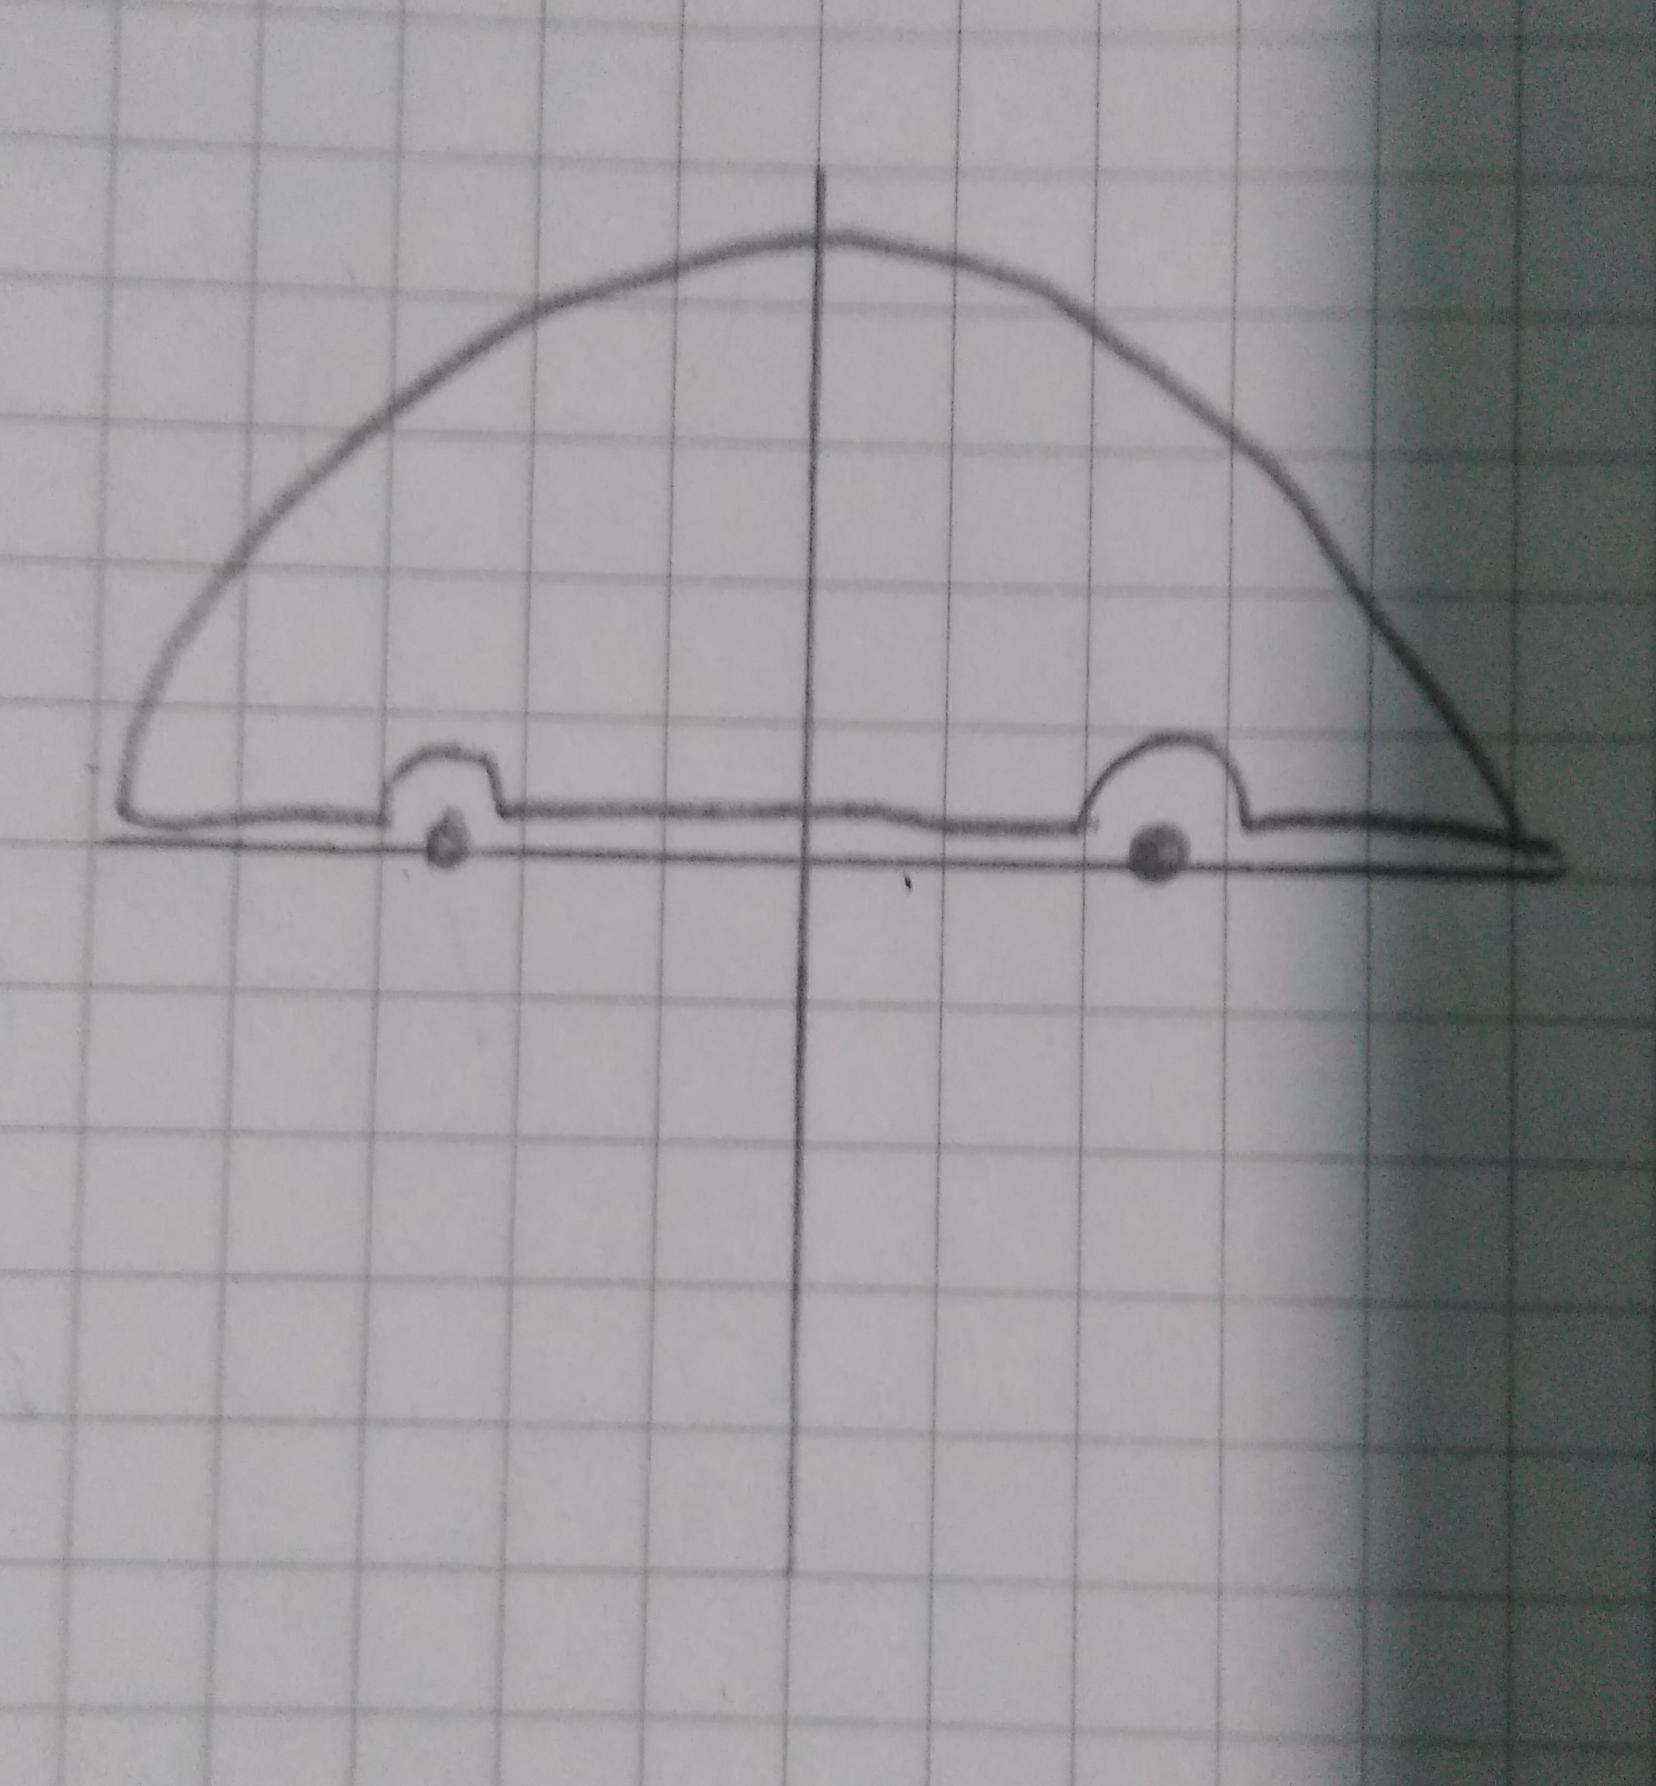
\includegraphics[width=0.4\textwidth]{Graficas/contorno_a.jpeg}
	    \caption{Contorno en el que se incluyen los dos polos por arriba}
	    \label{fig:contornoa}
	  \end{figure}

	  Ahora entonces con los polos encerrados esta integral queda:
	  \begin{align*}
	    \int_{c}&= 2\pi i\left( a^{\left( \sigma \right)}_{\left( -1 \right) }+a^{\left( -\sigma \right) }_{\left( -1 \right) } \right)  \\
	  .\end{align*}
	  Ahora si no los encerramos
	  \begin{align*}
	    \int_{c}&=\int_{-\infty}^{\infty}-\pi i \left( a^{\sigma}_{-1} + a^{-\sigma}_{-1} \right) = 0  \\
	  .\end{align*}

	  Ahora con esto podemos notar que es lo mismo con:
	  \begin{align*}
	    \int_{-\infty}^{\infty}=\pi i \left( a_{-1}^{\sigma} + a_{-1}^{-\sigma} \right) 
	  .\end{align*}

	\item En este caso por lema de Jordan una parte de la integral se cancele debemos usar el contorno en la imagen \ref{fig:contornob}
	  \begin{figure}[h]
	    \centering
	    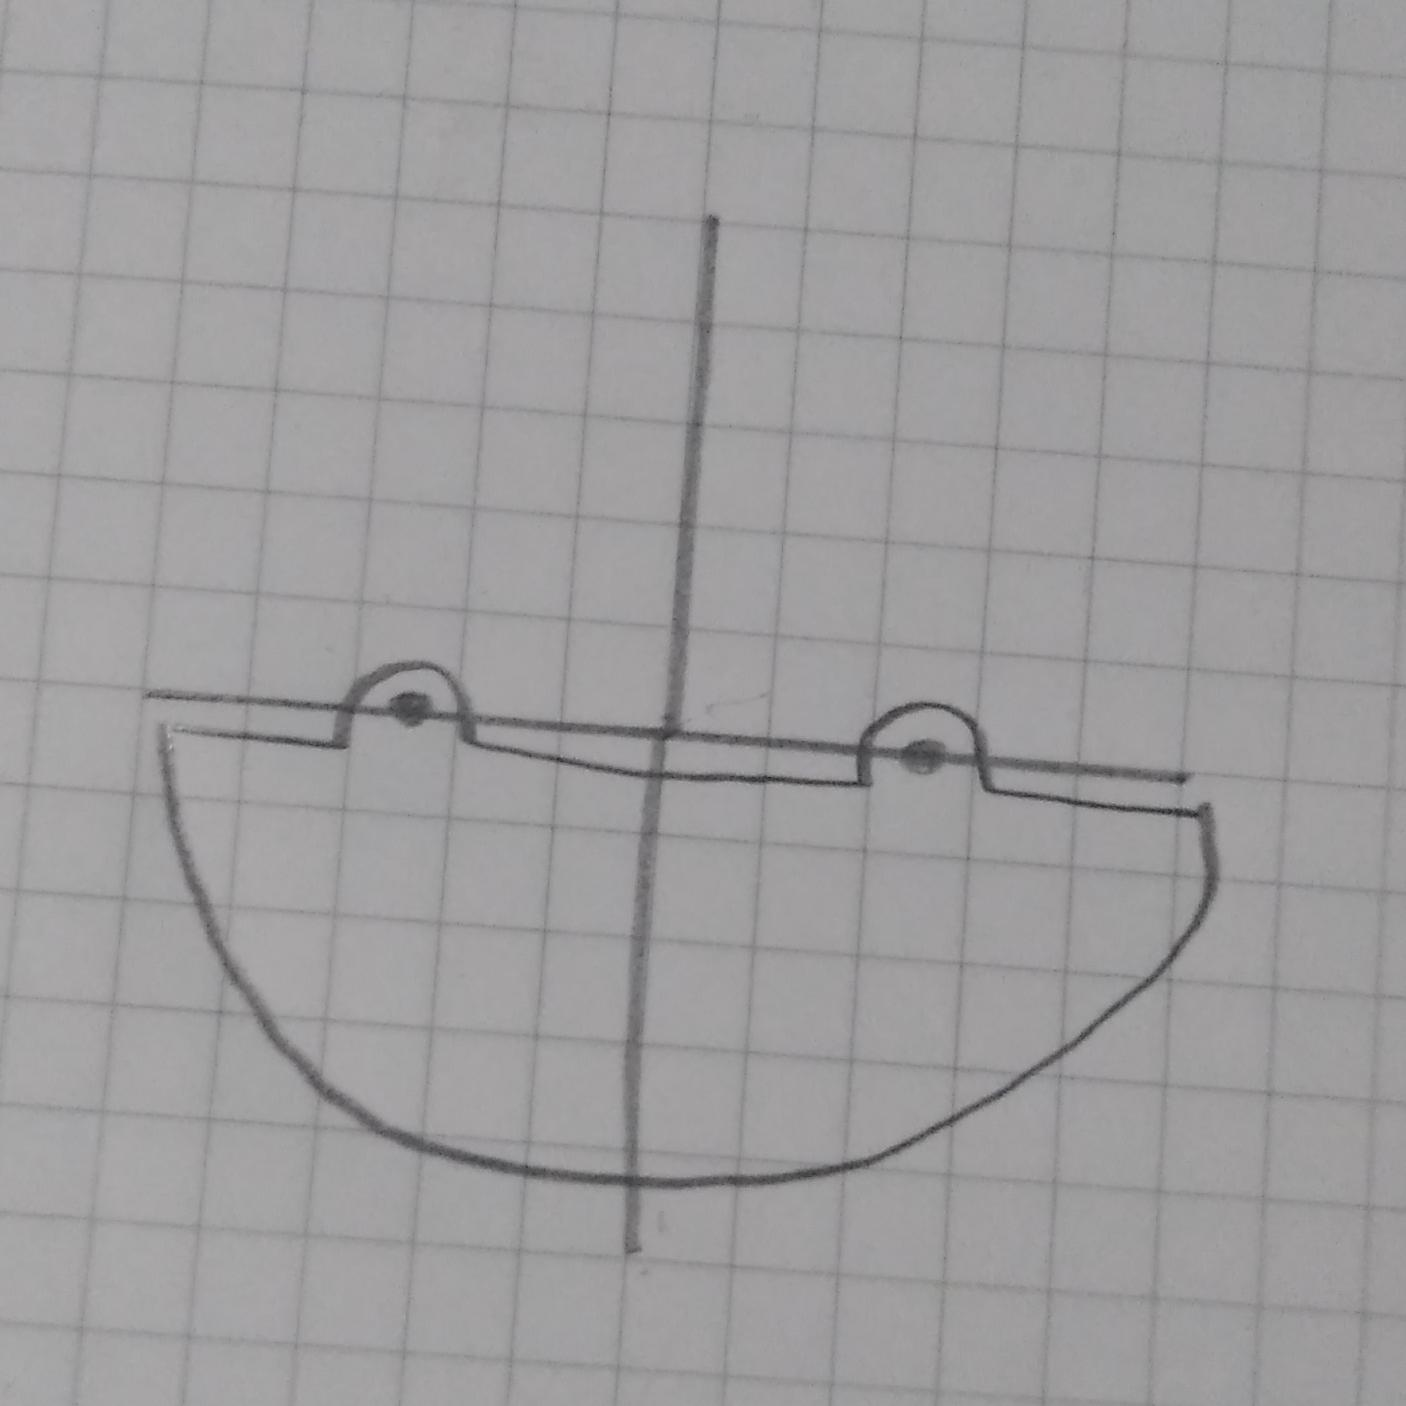
\includegraphics[width=0.4\textwidth]{Graficas/contorno_b.jpeg}
	    \caption{Contorno con el que se incluyen los polos por abajo}
	    \label{fig:contornob}
	  \end{figure}

	  ahora bien, la integral de los polos nos queda:
	  \begin{align*}
	    \int_{\sigma}+\int_{-\sigma}&= \pi i\left( a^{\sigma}_{-1}+ a^{\sigma}_{-1} \right)  \\
	  .\end{align*}

	  y con esto
	  \begin{align*}
	    \int_{-\infty}^{\infty}=-\pi i \left( a_{-1}^{\sigma} + a_{-1}^{-\sigma} \right) 
	  .\end{align*}
      \end{enumerate}
    \item Ahora vamos a evaluar cada integral
      \begin{align*}
        \int_{-\infty}^{\infty}\frac{xe^{ix}}{\left( x-\sigma \right) \left( x+\sigma \right) }dx &= \pi i \left( a^{\sigma}_{1}+a^{-\sigma}_{1} \right)  \\
	&= \pi i \left( \left( \frac{1}{0!}\left( \frac{ze^{iz}}{\left( z-\sigma \right) \left( z+\sigma \right) } \right)  \right) + \left( \frac{1}{0!}\left( \frac{ze^{iz}}{\left( z-\sigma \right) \left( z+\sigma \right) } \right)  \right)  \right)  \\
	&= \pi i \left( \frac{\sigma e^{i\sigma}}{2\sigma}+\frac{-\sigma e^{-i\sigma}}{-2\sigma} \right) = \pi i \left( \frac{e^{i\sigma} - e^{[i\sigma}}{2} \right) = \pi i \cos\left( \sigma \right) 
      .\end{align*}

      \begin{align*}
        \int_{-\infty}^{\infty}\frac{xe^{-ix}}{\left( x-\sigma \right) \left( x+\sigma \right) }dx &= \pi i \left( a^{sigma}_{-1}+a^{-\sigma}_{-1} \right)  \\
	&= - \pi i \cos\left( \sigma \right)  \\
      .\end{align*}
      \begin{align*}
        I\left( \sigma \right) = \frac{1}{2i}\left( \int_{-\infty}^{\infty}\frac{xe^{ix}}{\left( x-\sigma \right) \left( x+\sigma \right) }dx + \int_{-\infty}^{\infty}\frac{xe^{-ix}}{\left( x-\sigma \right) \left( x+\sigma \right) }dx\right) &= \frac{1}{2i}\left( \pi i\cos\left( \sigma \right) - \left( - \pi i \cos\left( \sigma \right)  \right)  \right)  \\
	&= \frac{2\pi i \cos\left( \sigma \right) }{2i} \\
	&= \pi \cos\left( \sigma \right) 
      .\end{align*}
    \item Ahora debemos hacer
      \begin{align*}
        \int_{-\infty}^{\infty}\frac{x\sin\left( x \right) }{x^2-\left( \sigma+i\epsilon \right)^2} dx &= \frac{1}{2i}\left( \int_{-\infty}^{\infty}\frac{xe^{ix}}{\left( x-\left( \sigma + i\epsilon \right)  \right) } dx - \int_{-\infty}^{\infty}\frac{xe^{-ix}}{\left( x-\left( \sigma+i\epsilon \right)  \right) \left( x-\left( -\sigma-i\epsilon \right)  \right) } dx \right) \\
      .\end{align*}

      y con esto trabajamos en cada integral $\sigma_{+}=\sigma + i\epsilon$ y $\sigma_{-}=\sigma - i\epsilon$

      \begin{align*}
	\int_{-\infty}^{\infty}\frac{xe^{ix}}{\left( x - \sigma_{+} \right) \left( x - \sigma_{-} \right) }dx &= 2\pi i \left( a_{-1}^{\sigma_{+}}+ a_{-1}^{\sigma_{-}} \right) \\
	&= 2\pi i \left( \left( \frac{\sigma_{+}e^{i\sigma_{+}}}{\sigma_{+}-\sigma_{-}} \right) + \left( \frac{\sigma_{-}e^{i\sigma_{-}}}{\sigma_{-}-\sigma_{+}} \right)  \right)  \\
	&= 2\pi i\left( \frac{\sigma_{+}e^{i\sigma_{+}}-\sigma_{-}e^{i\sigma_{-}}}{\sigma_{+}-\sigma_{-}} \right)  \\
	&= 2\pi i \frac{\sigma_{+}\left( e^{i\sigma_{+}}+e^{i\sigma_{-}} \right) }{2\sigma_{+}} \\
	&= 2\pi i \cos\left( \sigma_{+} \right)
      .\end{align*}

      \begin{align*}
	\int_{-\infty}^{\infty}\frac{xe^{-ix}}{\left( x-\sigma_{+} \right) \left( x-\sigma_{-} \right) } dx &= -2\pi i\left( a_{-1}^{\sigma_{+}}+a_{-1}^{\sigma_{-}} \right)  \\
	&= -2\pi i\cos\left( \sigma_{+} \right)
      .\end{align*}

      \begin{align*}
        \frac{1}{2i}\left( \int_{-\infty}^{\infty}\frac{xe^{ix}}{\left( x-\sigma_{+} \right) \left( x-\sigma_{-} \right) }dx - \int_{-\infty}^{\infty}\frac{xe^{-ix}}{\left( x-\sigma_{+} \right) \left( x-\sigma_{-} \right) } \right) &= \frac{1}{2i}\left( 2 \pi i \cos\left( \sigma_{+} \right) - \left( -2\pi i \cos\left( \sigma_{+} \right)  \right)  \right)  \\
	&= \frac{1}{2i}4\pi i\cos\left( \sigma_{+} \right)  \\
	&= 2\pi \cos\left( \sigma_{+} \right)  \\
	&= 2\pi \cos\left( \sigma + i\epsilon \right)
      .\end{align*}
  \end{enumerate}

  \chapter{}
  
  \begin{align*}
    \int_{-\infty}^{\infty}\frac{\cos\left( mx \right) }{x^2+x+2}dx=\int_{-\infty}^{\infty}\frac{e^{imx}+e^{-imx}}{2\left( x^2+x+2 \right) }
  .\end{align*}

  para lo cual
  \begin{align*}
    x^2+x+2&= 0 \\
    x &= \frac{-1\pm\sqrt{1^2-4\left( 2 \right) } }{2} \\
    &= \frac{1}{2}\left( -1 \pm i\sqrt{7}  \right)  \\
    z_{+} &= \frac{1}{2}\left( -1+i\sqrt{7}  \right)  \\
    z_{-} &= \frac{1}{2}\left( -1-i\sqrt{7}  \right)
  .\end{align*}

  \begin{align*}
    \int_{-\infty}^{\infty}\frac{e^{imx}}{2\left( x^2+x+2 \right) }dx &= \frac{1}{2}\int_{-\infty}^{\infty} \frac{e^{imx}}{\left( x-z_{+} \right) \left( x-z_{-} \right) }dx \\
    &= \frac{1}{2}\left( 2\pi ia^{z_{+}}_{-1} \right) =\left( \pi i \right) \left( \frac{1}{\left( 1-1 \right)!} \right) \left( \frac{z-z_{+}}{1}\cdot \frac{e^{imz}}{\left( z-z_{+} \right) \left( z-z_{-} \right) } \right)  \\
    &= \pi i \frac{e^{imz_{+}}}{\left( z_{+}-z_{-} \right) } \\
    &= \frac{\pi i e^{imz_{+}}}{i\sqrt{7} } \\
    &= \frac{\pi}{\sqrt{7} }\frac{1}{e^{\frac{im}{2}}e^{\frac{\sqrt{7} m}{2}}}
  .\end{align*}

  \begin{align*}
    \int_{-\infty}^{\infty}\frac{e^{-imx}}{2\left( x^2+x+2 \right) }dx &= \frac{1}{2}\int_{-\infty}^{\infty}\frac{e^{-imx}}{\left( x-z_{+} \right) \left( x-z_{-} \right) } \\
    &= -\pi i\left( \frac{e^{-imz}}{\left( z-z_{+} \right) \left( z-z_{-} \right) } \right)  \\
    &= -\pi i \frac{e^{im \frac{1}{2}+i^2m \frac{\sqrt{7} }{2}}}{-zi \sqrt{\frac{7}{4}} } \\
    &= \frac{\pi}{\sqrt{7} }\frac{e^{im \frac{1}{2}}}{e^{m \frac{\sqrt{7} }{2}}}
  .\end{align*}

  Ahora sumamos ambas integrales:
  \begin{align*}
    \int_{-\infty}^{\infty}\frac{e^{imx}}{2\left( x^2+x+2 \right) }dx + \int_{-\infty}^{\infty}\frac{e^{-imx}}{2\left( x^2+x+2 \right) }dx\\
    =\frac{\pi}{\sqrt{7} }\frac{1}{e^{\frac{im}{2}}e^{\frac{\sqrt{7} m}{2}}}+ \frac{\pi}{\sqrt{7} }\frac{e^{im \frac{1}{2}}}{e^{\frac{\sqrt{7} m}{2}}}\\
    =\frac{\pi}{\sqrt{7} e^{\frac{\sqrt{7} m}{2}}}\left( e^{-\frac{im}{2}}+e^{\frac{im}{2}} \right) \\
    =\frac{\pi}{\sqrt{7} e^{\sqrt{7} \frac{m}{2}}}2\cos\left( \frac{m}{2} \right) 
  .\end{align*}
\end{document}
